\begin{figure*}
\centering
\subfloat[]{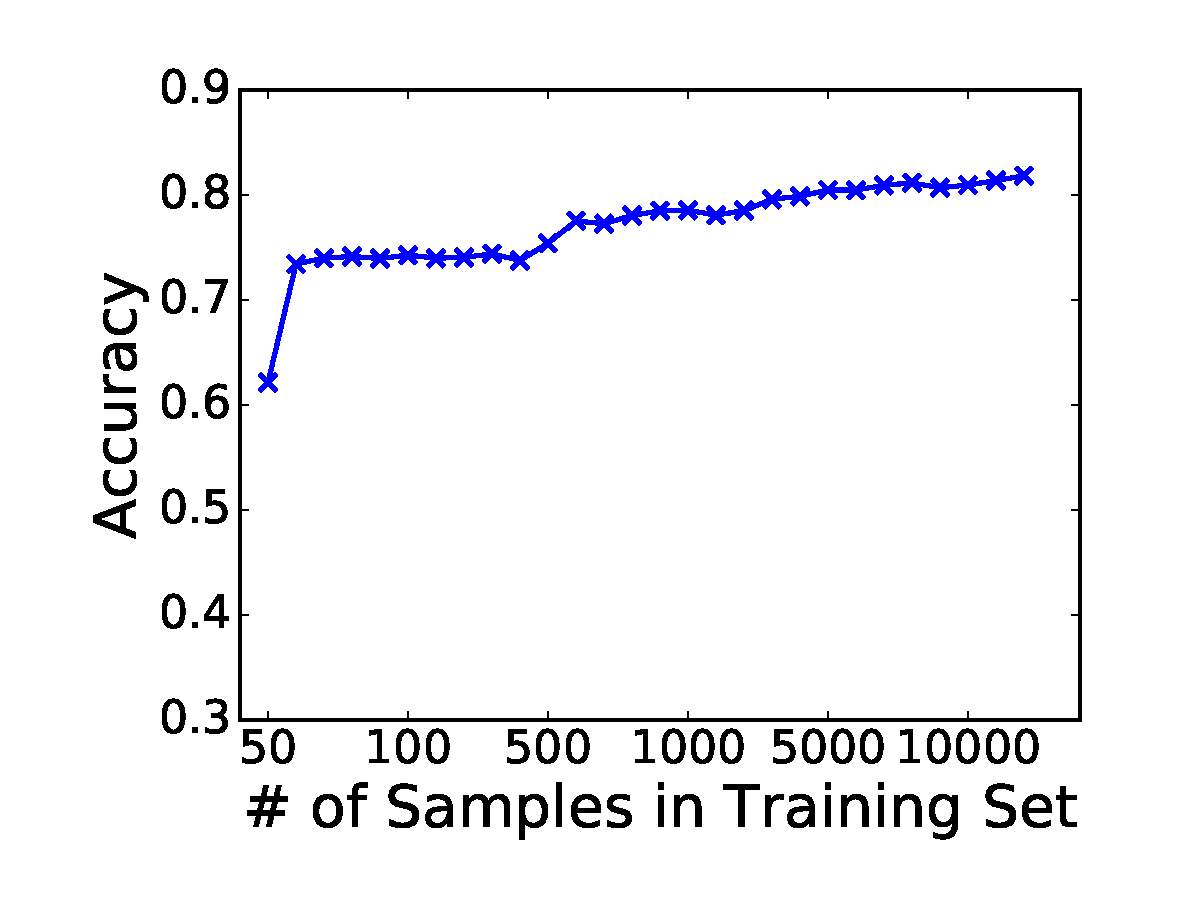
\includegraphics[width=0.16\linewidth]{figure/svm/0}\label{fig:moredata1}} 
\subfloat[]{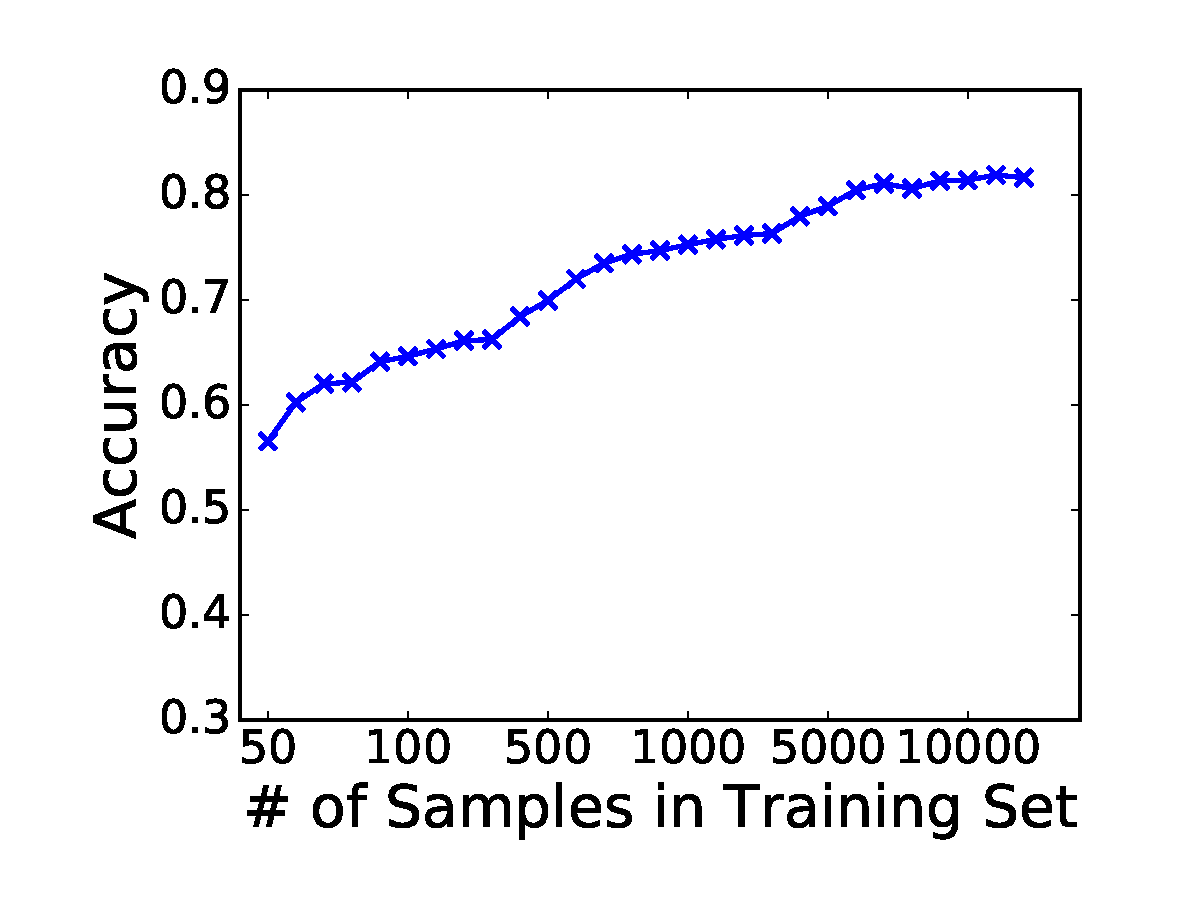
\includegraphics[width=0.16\linewidth]{figure/svm/1}\label{fig:moredata2}}
\subfloat[]{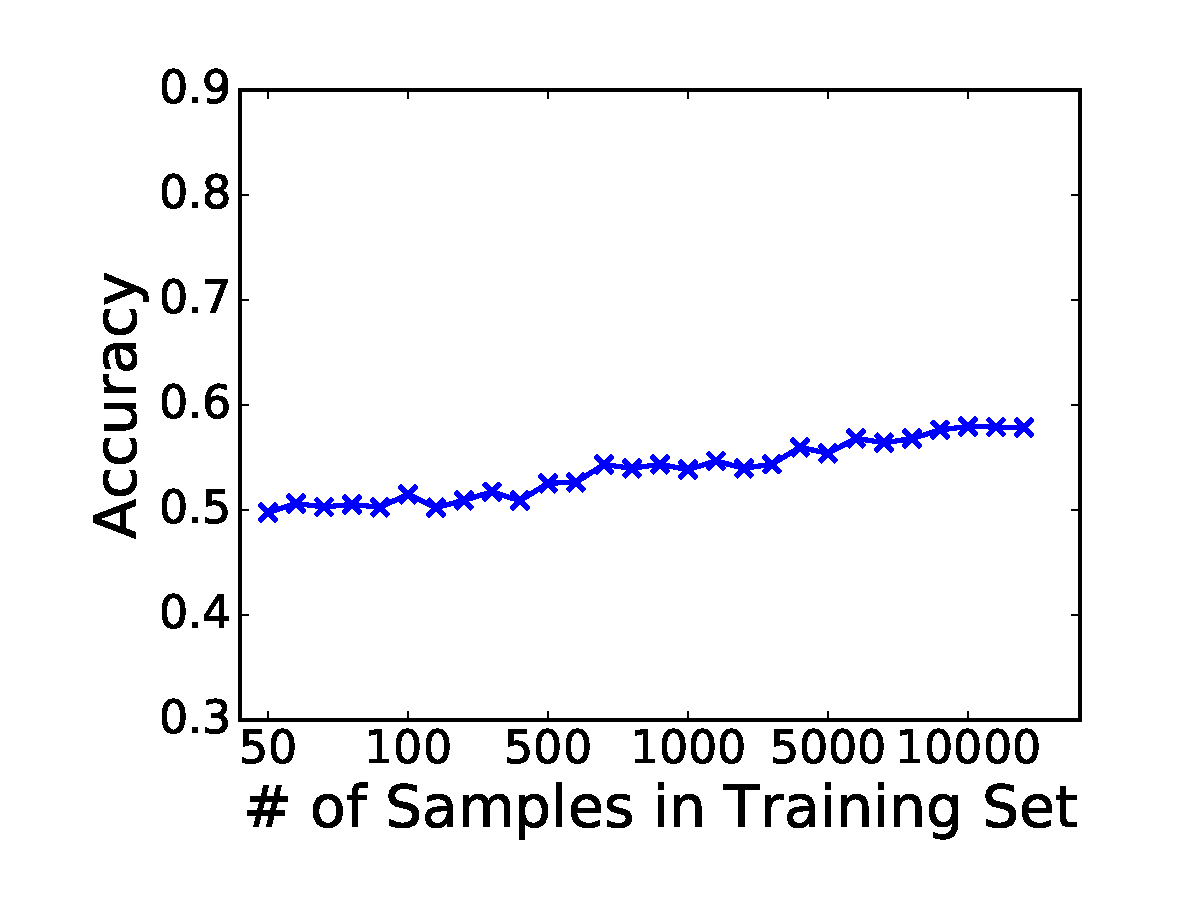
\includegraphics[width=0.16\linewidth]{figure/svm/2}\label{fig:moredata3}} 
\subfloat[]{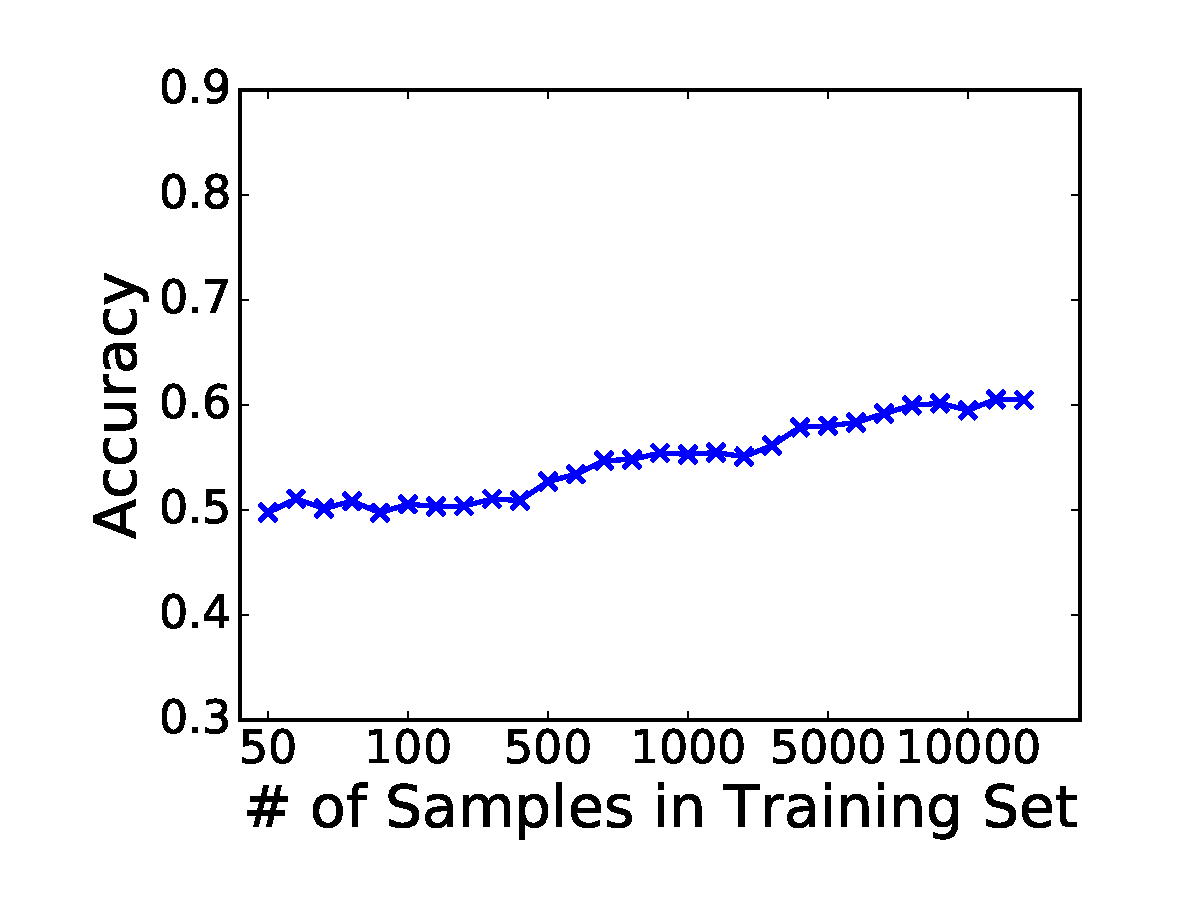
\includegraphics[width=0.16\linewidth]{figure/svm/3}\label{fig:moredata4}}
\subfloat[]{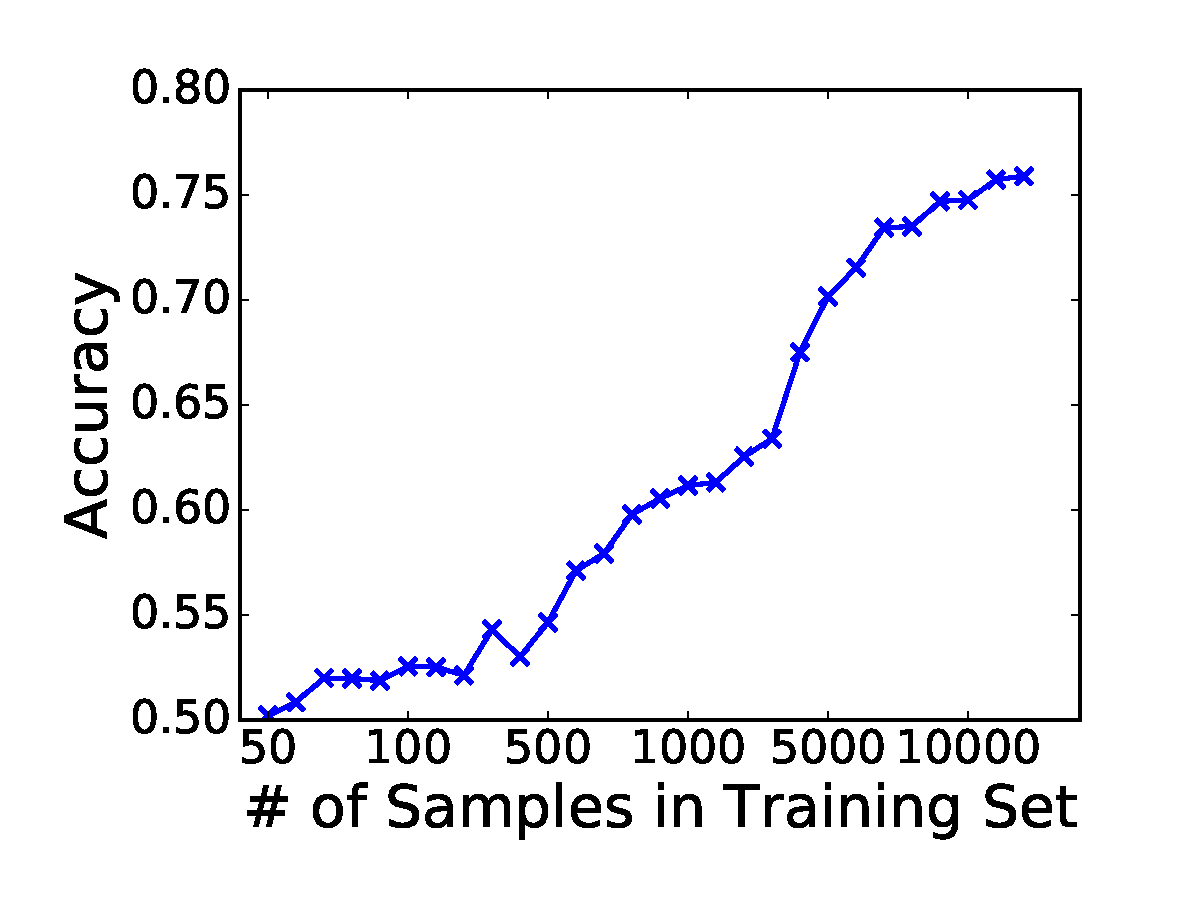
\includegraphics[width=0.16\linewidth]{figure/svm/4}\label{fig:moredata5}} \\ 

\subfloat[]{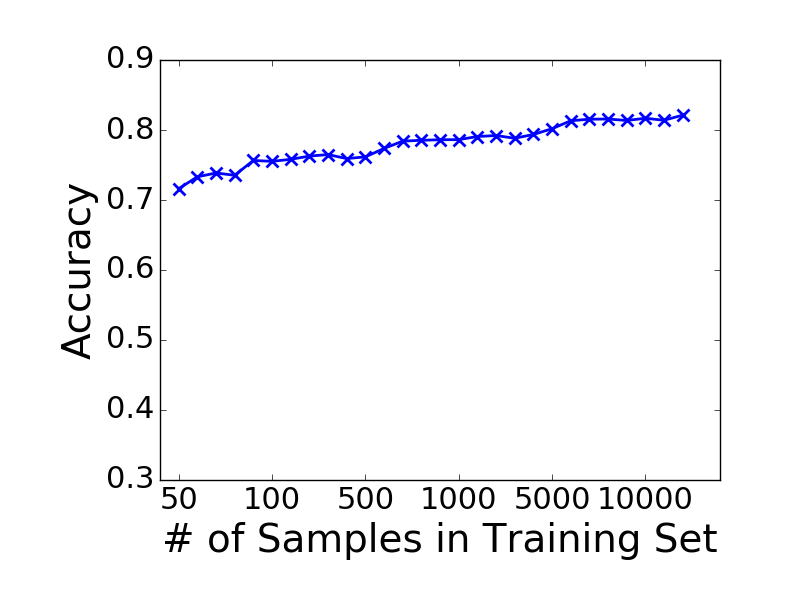
\includegraphics[width=0.16\linewidth]{figure/svm/5}\label{fig:moredata6}} 
\subfloat[]{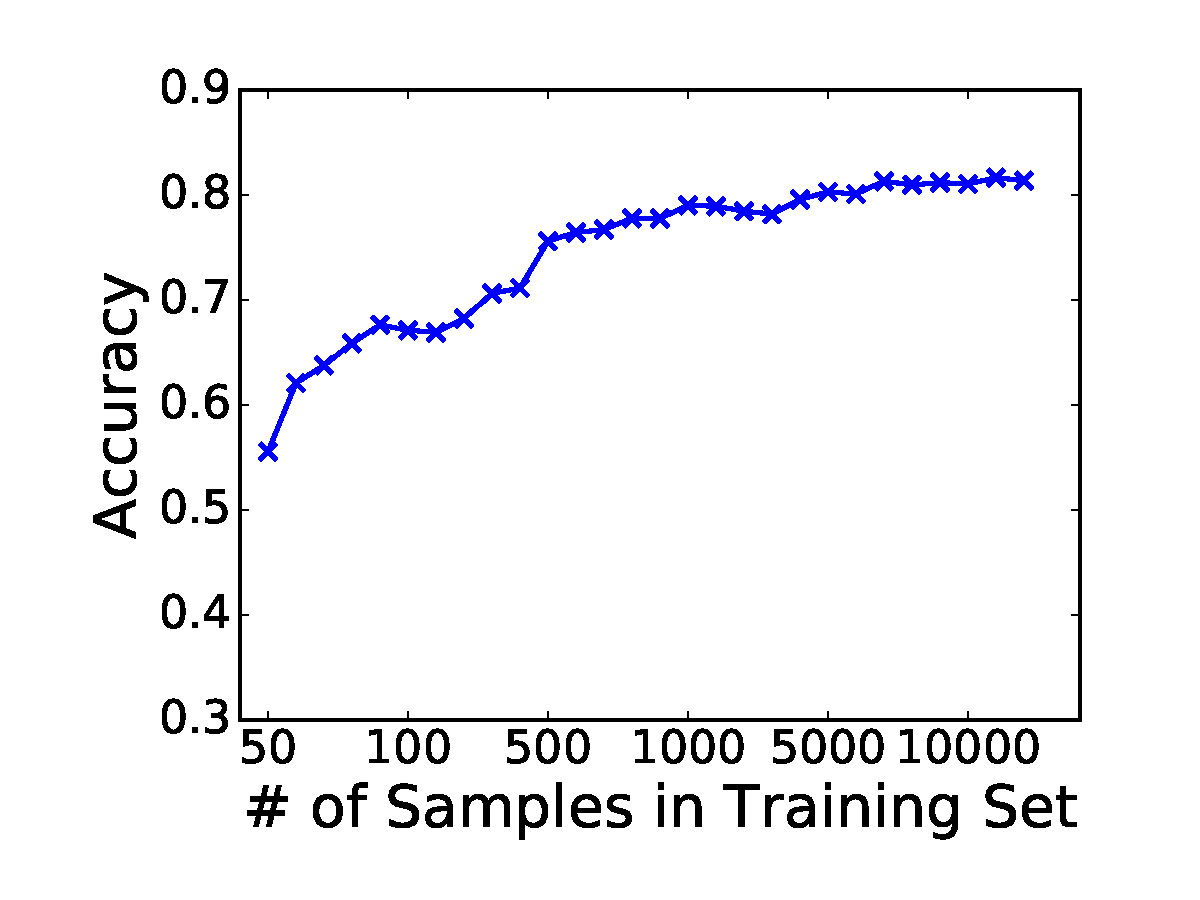
\includegraphics[width=0.16\linewidth]{figure/svm/6}\label{fig:moredata7}}
\subfloat[]{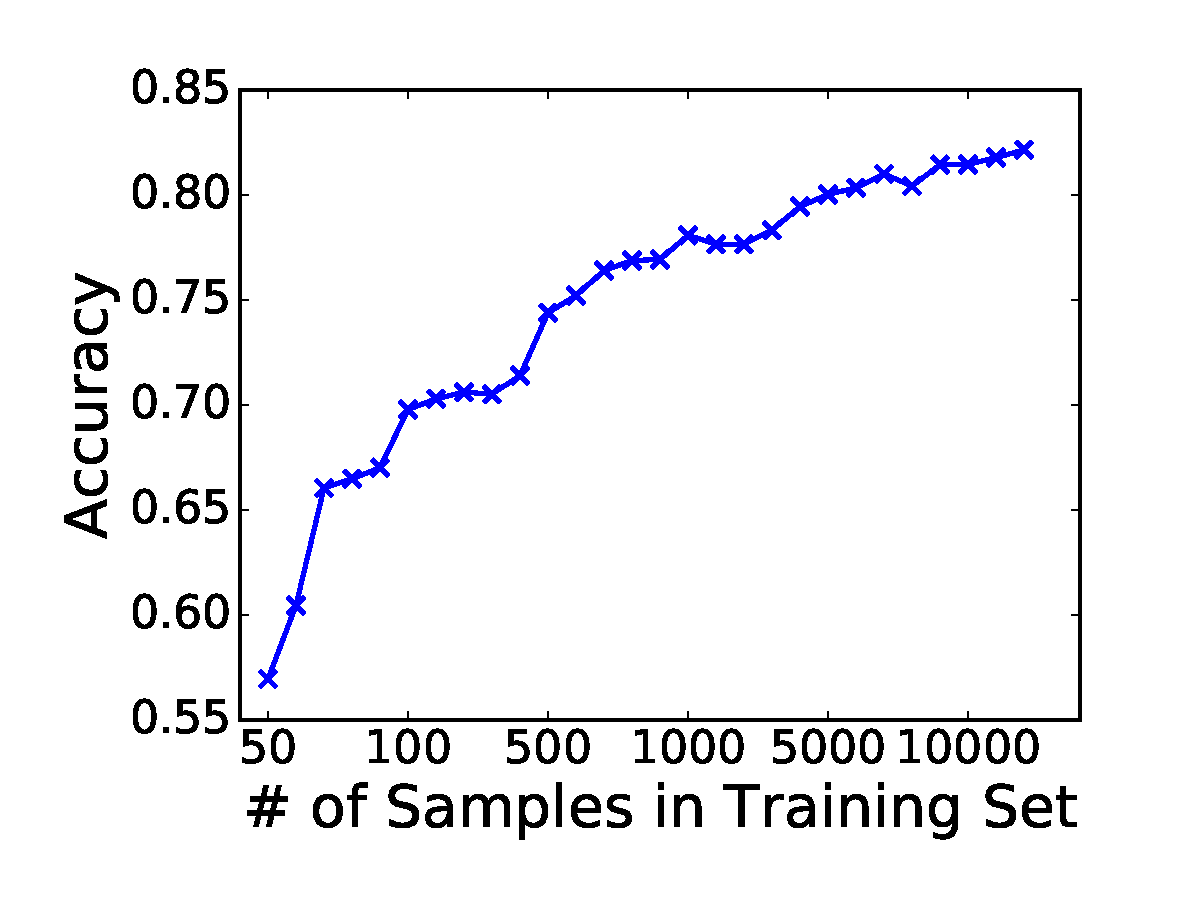
\includegraphics[width=0.16\linewidth]{figure/svm/7}\label{fig:moredata8}} 
\subfloat[]{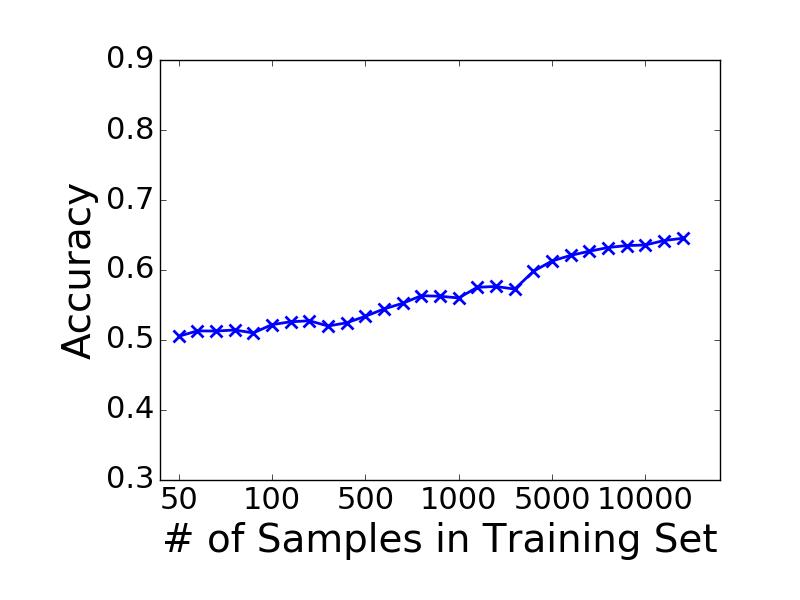
\includegraphics[width=0.16\linewidth]{figure/svm/8}\label{fig:moredata9}}
\subfloat[]{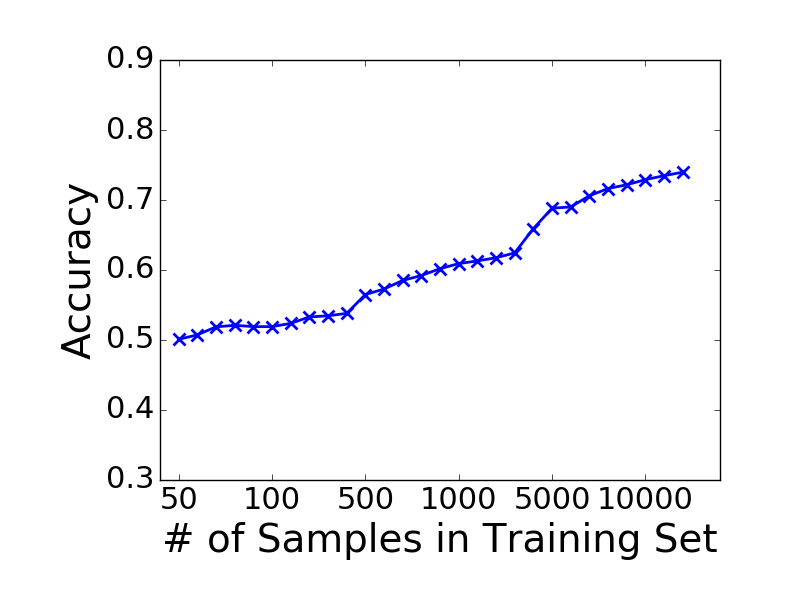
\includegraphics[width=0.16\linewidth]{figure/svm/9}\label{fig:moredata10}}
\subfloat[]{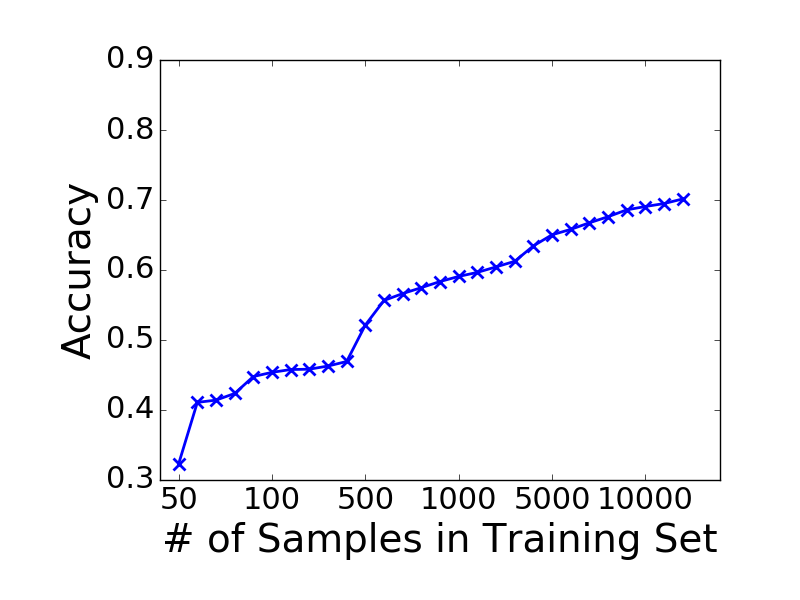
\includegraphics[width=0.16\linewidth]{figure/svm/10}\label{fig:moredata11}}
\caption{\ce{LINHAI, CHANGE THE TITLE AND EXPLAIN WHAT (A)-(K) IS} Heat Maps for Learned Models. 
{\footnotesize{(Heat maps drawn for $p_{u,v}$ tables of the 4 models. 
$Cell(u,v)$ contains influence probability from $u$ to $v$, where $u$ is row number, and $v$ is column number.
A larger number means more influence from $u$ to $v$. )}}} 
\label{fig:moredata} 
\end{figure*} 